\chapter{Clean Architecture}
Bei der Umsetzung des Softwareentwurfs wurde sich an der Theorie der Clean Architecture orientiert.
Im folgenden Kapitel wird die Planung der einzelnen Schichten beschrieben sowie die Anwendung der Schichten auf den Programmentwurf.

\section{Planung der Schichten}
Das Ziel der Clean Architecture ist das Erstellen einer langfristigen Software-Architektur.
Schließlich werden während eines Lebenszykluses einer Software unterschiedliche Technologien auf dem Markt angeboten.
Diese Technologien können unterschiedliche Anwendungsfälle haben.
Dazu zählt zum Beispiel die Datenbanktechnologie sowie die dazugehörige Anbindung an das Softwaresystem oder auch die Technologie der grafischen Oberfläche.
Somit bedarf es der Möglichkeit, mit möglichst geringem Aufwand eingesetzte Technologien auszutauschen.
Ist die Softwarearchitektur nun an die verwendeten Technologien gebunden, dann ist ein Austauschen der Technologie nur schwer möglich und bedarf großem Aufwand an mitunter vielen Stellen innerhalb der Software.

Zur Minimierung dieses Aufwands durch einen Technologieaustausch, setzt die Clean Architecture grundsätzlich auf einen bestimmten Aufbau.
Zunächst besitzt die Anwendung einen technologieabhängigen Kern, der die eigentlichen Geschäftsregeln enthält.
Darauf folgt jede Abhängigkeit als temporäre Lösung, das heißt, dass eine Abhängigkeit von den Geschäftsregeln als temporäre Lösung realisiert ist.
Ein Entfernen der Abhängigkeit führt somit nicht dazu, dass das Programm nicht mehr kompiliert werden kann.
Man teilt daher auch in zentralen und somit langlebigen Code sowie peripherem, oder auch kurzfristigem, Sourcecode ein.
Den innersten Kern bietet der \textit{Abstraction Code}. 
Er enthält domänenübergreifendes Wissen. 
Dazu zählen beispielsweise mathematische Konzepte oder phyisikalische Grundlagen.
Eine Änderung dieses Wissens ist nahezu ausgeschlossen.
Darauf folgt der \textit{Domain Code}.
Er enthält die Entitäten der Anwendungen und somit die eigentliche organisationsweite Geschäftslogik.
Der \textit{Domain Code} sollte sich am seltestenen ändern.
Als nächste Schicht folgt der \textit{Application Code}.
Darin ist die Applikationslogik beziehungsweise die anwendungsspezifische Geschäftslogik enthalten, welche mit den Entitäten aus dem \textit{Domain Code} angewandt wird.
Eine Änderung dieses Codes ist möglich, wenn sich die Anforderungen der Software ändern.
Auf den \textit{Application Code} folgt die \textit{Adapters}-Schicht.
Diese Schicht dient als Interface für Adapter und enthält daher nötige Controller, Presenters oder Gateways.
Die Schicht fungiert als Zwischenschicht und vermittelt Aufrufe sowie Daten an die innere Schichten.
Das Ziel ist dabei die Entkopplung der inneren und äußeren Schichten, weshalb man auch von einem \textit{Anti Corruption Layer} spricht.
Als letzte Schicht folgen die \textit{Plugins}.
Darin enthalten sind eingesetzte Frameworks oder Treiber.
Diese Schicht ist vor allem für die Anbindung an eine Datenbank, die grafische Oberfläche oder auch Drittsysteme nötig.
\textit{Plugins}-Code greift eher nur auf die \textit{Adapters}-Schicht zu und ist leicht auszutauschen.

Der Aufbau der Architektur entspricht somit einer Zwiebel und wird daher auch \textit{Onion Architecture} bezeichnet.

Wichtig ist bei diesem Aufbau, dass jeweilige Abhängigkeiten nur in tieferliegende Schichten bestehen dürfen.
Innere Schichten dürfen daher die äußeren Schichten nicht kennen.
Man bezeichnet diese Regel auch als \textit{Dependency Rule}.
Eine Anwendung der \textit{Dependency Injection} sowie \textit{Dependency Inversion} kann hierbei unterstützen.
Das Ziel ist dadurch, dass ein Austausch einer Technologie somit nur die äußerste Schicht betrifft, der Kern der Software hiervon jedoch unberührt ist und somit die Geschäftslogik nicht davon beeinflusst.
Somit wird es möglich, dass Code nur von langlebigerem Code als sich selbst abhängig ist.

Die Grenzen der Clean Architecture ist allerdings, dass technische Grundlagen dennoch gegeben und stabil sein müssen.
Dazu zählt die verwendete Programmiersprache, der Compiler und die Laufzeitumgebung sowie auch in gewissem Maße das Betriebssystem oder die eingesetzte Hardware.
Frameworks können diese Grenzen ebenfalls einschränken, wenn eine zu starke Bindung stattfindet.
Dieser Eingrenzung muss man sich bei der Planung der Software-Architektur im Klaren sein und daraus mögliche Folgen erkennen beziehungsweise abwägen.

\section{Anwendung der Schichten}
Im Folgenden wird die Umsetzung der \textit{Clean Architecture} innerhalb dieses Softwareentwurfs beschrieben.

Zunächst ist die Projektstruktur entsprechend realisiert worden.
Anstatt alle nötigen Klassen in einem Projekt zu erzeugen, ist zur Übersichtlichkeit eine Strukturierung entsprechend der Schichten vorgenommen worden.
Die Strukturierung der einzelnen Schichten ist nicht über Packages gemacht worden.
Diese Variante ist grundsätzlich möglich, jedoch findet dabei keine Überprüfung durch den Compiler statt und es ist somit schwieriger möglich, einzelne Abhängigkeiten von innen nach außen zu erkennen.
Stattdessen bietet sich die Form mehrerer Projekte an.
Jedes Projekt bildet dabei eine Schicht ab.
Der Compiler erkennt nun nur die im eigenen Projekt sowie in referenzierten Projekten vorhandene Klassen.
Diese Möglichkeit unterstützt bei der Umsetzung der tiefergehenden Abhängigkeiten.
Darüber hinaus dient ein Überprojekt als Abbild des gesammten Projekts und der Klammerung der einzelnen Schicht.
Abbildung \ref{fig:projektstruktur} zeigt die umgesetzte Projektstruktur und Abbildung \ref{fig:umsetzung-pom} die pom.xml zur Umsetzung der einzelnen Projekte in einem Klammerprojekt.
Die einzelnen Projekte, die jeweils eine Schicht der \textit{Clean Architecture} abbilden, sind in dieses globale Projekt als Module eingebunden.

\begin{figure}[H]
	\centering
	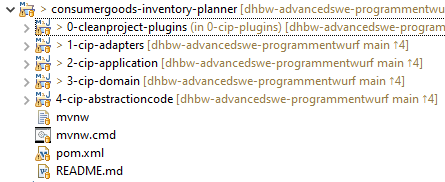
\includegraphics[width=1.0\textwidth]{Bilder/projektstruktur.PNG}
	\caption[Aufteilung der Projektstruktur entsprechend \textit{Clean Architecture}.]{Die Projektstruktur ist entsprechend der \textit{Clean Architecture} in einzelne Unterprojekte aufgeteilt.}
	\label{fig:projektstruktur}
\end{figure}

\begin{figure}[H]
	\centering
	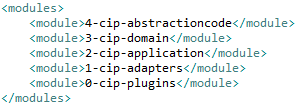
\includegraphics[width=1.0\textwidth]{Bilder/ausschnitt-pom.PNG}
	\caption[Ausschnitt aus der pom.xml zur Projektstruktur.]{Der Ausschnitt zeigt die Umsetzung der Projektstruktur zwischen dem Klammerprojekt und den einzelnen Unterprojekten.}
	\label{fig:umsetzung-pom}
\end{figure}

Die Realisierung der einzelnen Schichten bezieht sich auf den Anwendungsbezug und die Anforderungen der Anwendung.
Das zum Programmentwurf dazugehörige \href{https://github.com/lucasmerkel/dhbw-advancedswe-programmentwurf/blob/d5c89113d12c3b877ddc4d6a99225b277ddd468f/Documentation/Bilder/uml-diagramme/klassendiagramm.svg}{\code{Klassendiagramm}} verdeutlicht farblich die Zugehörigkeit der Klasen entsprechend der \textit{Clean-Architecture}.
Die farbliche Zuordnung ist wie folgt:
\begin{itemize}
    \item weiß entspricht der \textit{Abstraction Code}-Schicht,
    \item dunkelblau der \textit{Domain Code}-Schicht,
    \item hellblau der \textit{Application Code}-Schicht,
    \item dunkelgrün der \textit{Adapter Code}-Schicht und
    \item hellgrün der \textit{Plugin Code}-Schicht.
\end{itemize}

%\begin{figure}[H]
%	\centering
%	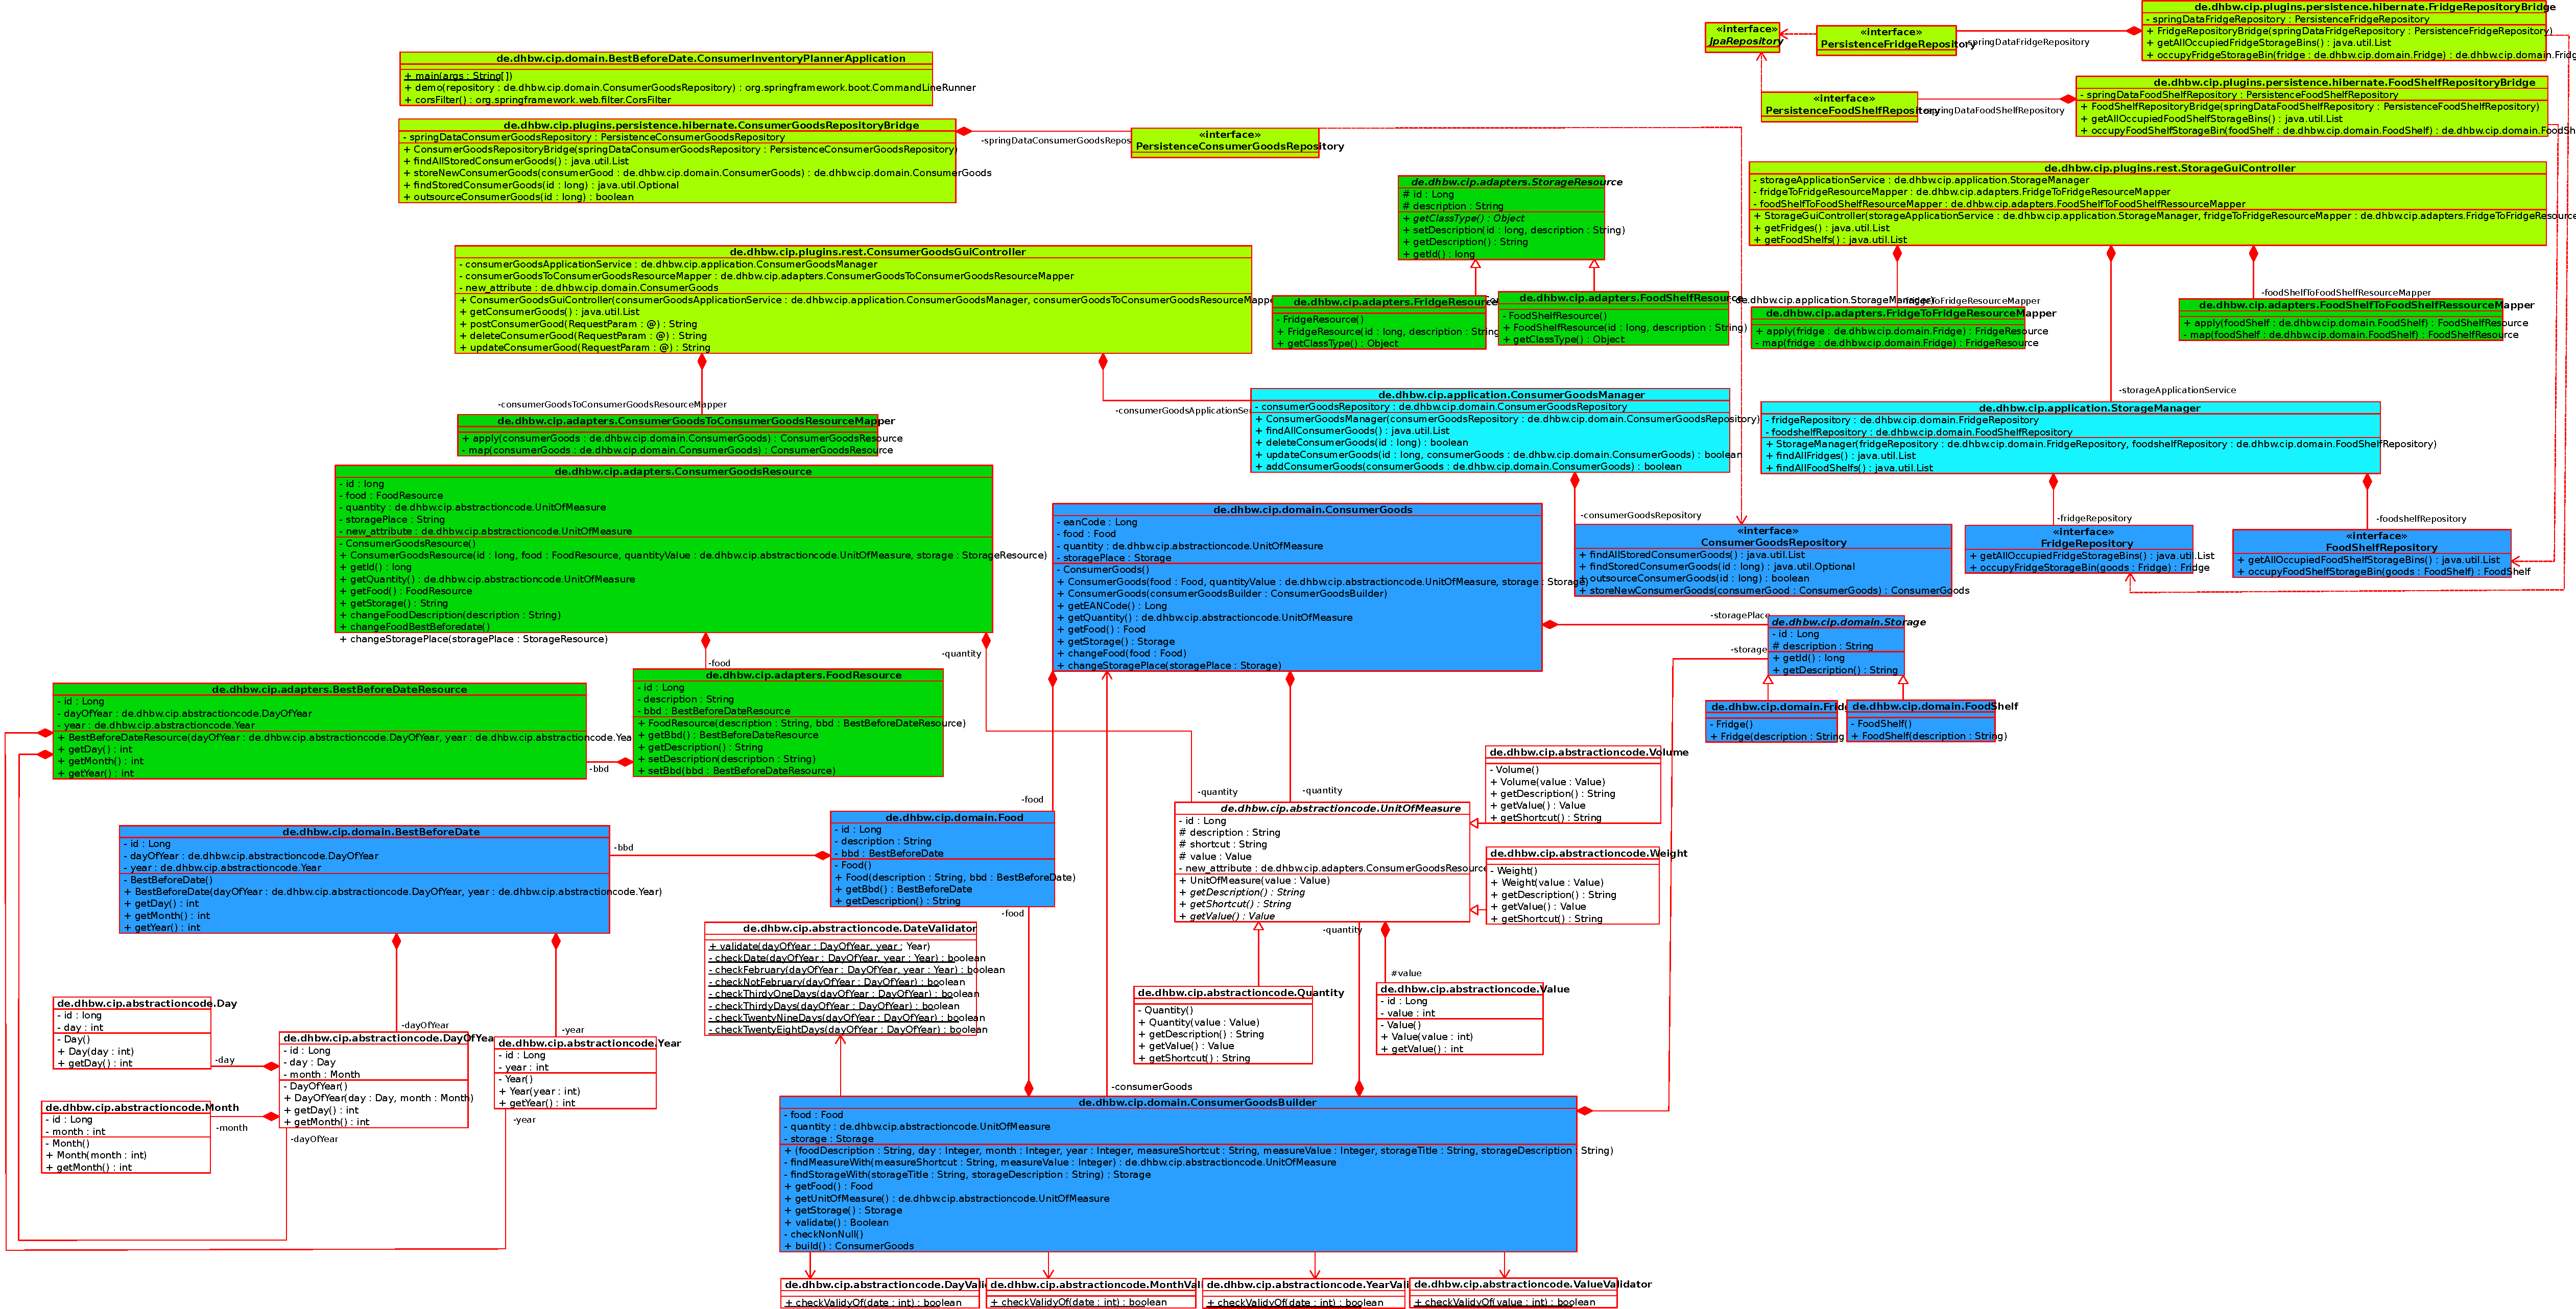
\includegraphics[width=1.0\textwidth]{Bilder/class diagram.pdf}
%	\caption[UML-Diagramm des Software-Entwurfs.]{Das UML-Diagramm des Software-Entwurfs mit entsprechend der \textit{Clean Architecture} farblich kategorisierten Klassen.}
%	\label{fig:uml-diagramm}
%\end{figure}

Die Software dient als \ac{REST}-Server zur Verwaltung der Lebensmittel Zuhause.
Dabei können Lebensmittel sowohl im Kühlschrank, der Gefriertruhe oder in einem Regal gelagert werden.
Neue Lebensmittel können angelegt werden.
Dabei ist die Bezeichnung des Lebensmitttels sowie die entsprechende Menge und das Mindesthaltbarkeitsdatum relevant.
Bei fehlerhafter Eingabe oder dem teilweisen Verbrauch können entsprechende Werte angepasst werden.
Verbrauchte Lebensmittel können gelöscht werden.
Dementsprechend sieht eine Umsetzung der einzelnen Schichten wie folgt aus:

\subsection*{\textit{Abstraction Code}-Schicht}
In der \href{https://github.com/lucasmerkel/dhbw-advancedswe-programmentwurf/tree/main/swe_programmentwurf/consumergoods-inventory-planner/4-cip-abstractioncode}{\code{Abstraction Code}}-Schicht befinden sich Klassen für die Verwaltung der Maßeinheit der Lebensmittel.
Die Klasse \href{https://github.com/lucasmerkel/dhbw-advancedswe-programmentwurf/blob/d5c89113d12c3b877ddc4d6a99225b277ddd468f/swe_programmentwurf/consumergoods-inventory-planner/4-cip-abstractioncode/src/main/java/de/dhbw/cip/abstractioncode/UnitOfMeasure.java}{\code{UnitOfMeasure}} ist die Superklasse der Subklassen \href{https://github.com/lucasmerkel/dhbw-advancedswe-programmentwurf/blob/d5c89113d12c3b877ddc4d6a99225b277ddd468f/swe_programmentwurf/consumergoods-inventory-planner/4-cip-abstractioncode/src/main/java/de/dhbw/cip/abstractioncode/Quantity.java}{\code{Quantity}}, \href{https://github.com/lucasmerkel/dhbw-advancedswe-programmentwurf/blob/d5c89113d12c3b877ddc4d6a99225b277ddd468f/swe_programmentwurf/consumergoods-inventory-planner/4-cip-abstractioncode/src/main/java/de/dhbw/cip/abstractioncode/Volume.java}{\code{Volume}} sowie \href{https://github.com/lucasmerkel/dhbw-advancedswe-programmentwurf/blob/d5c89113d12c3b877ddc4d6a99225b277ddd468f/swe_programmentwurf/consumergoods-inventory-planner/4-cip-abstractioncode/src/main/java/de/dhbw/cip/abstractioncode/Weight.java}{\code{Weight}}.
Diese Klassen repräsentieren die zugehörige Maßeinheit. Der entsprechende Wert wird durch eine Referenz auf ein Objekt der Klasse \href{https://github.com/lucasmerkel/dhbw-advancedswe-programmentwurf/blob/d5c89113d12c3b877ddc4d6a99225b277ddd468f/swe_programmentwurf/consumergoods-inventory-planner/4-cip-abstractioncode/src/main/java/de/dhbw/cip/abstractioncode/Value.java}{\code{Value}} gespeichert.
Gleiches gilt für die Repräsentation des Datums eines Tages, Monats und Jahres.
Dafür dienen die Klassen \href{https://github.com/lucasmerkel/dhbw-advancedswe-programmentwurf/blob/d5c89113d12c3b877ddc4d6a99225b277ddd468f/swe_programmentwurf/consumergoods-inventory-planner/4-cip-abstractioncode/src/main/java/de/dhbw/cip/abstractioncode/Day.java}{\code{Day}}, \href{https://github.com/lucasmerkel/dhbw-advancedswe-programmentwurf/blob/d5c89113d12c3b877ddc4d6a99225b277ddd468f/swe_programmentwurf/consumergoods-inventory-planner/4-cip-abstractioncode/src/main/java/de/dhbw/cip/abstractioncode/Month.java}{\code{Month}} sowie \href{https://github.com/lucasmerkel/dhbw-advancedswe-programmentwurf/blob/d5c89113d12c3b877ddc4d6a99225b277ddd468f/swe_programmentwurf/consumergoods-inventory-planner/4-cip-abstractioncode/src/main/java/de/dhbw/cip/abstractioncode/Year.java}{\code{Year}}.
Die Klassen für die Maßeinheit und die Repräsentation eines Tages, eines Monats sowie eines Jahres sind in dieser Schicht festgelegt, da die Informationsrepräsentation der Klassen auf domänenübergreifendes Wissen zurückzuführen ist, dessen Änderung und somit auch das der Klassen ausgeschlossen.
Die Klassen benötigen zudem keine Abhängigkeit zu Klassen der äußeren Schichten.

\subsection*{\textit{Domain Code}-Schicht}
Die \href{https://github.com/lucasmerkel/dhbw-advancedswe-programmentwurf/tree/main/swe_programmentwurf/consumergoods-inventory-planner/3-cip-domain}{\code{Domain Code}}-Schicht enthält die für den Anwendungsfall der Software relevanten Domänen.
Dazu zählt zum einen die Klasse \href{https://github.com/lucasmerkel/dhbw-advancedswe-programmentwurf/blob/main/swe_programmentwurf/consumergoods-inventory-planner/3-cip-domain/src/main/java/de/dhbw/cip/domain/ConsumerGoods.java}{\code{ConsumerGoods}}.
Diese Klasse dient der Repräsentation der Lebensmittel als einer der Domänen.
Innerhalb der Klasse \href{}{\code{}}\code{ConsumerGoods} werden dabei die weiteren Klassen \href{https://github.com/lucasmerkel/dhbw-advancedswe-programmentwurf/blob/d5c89113d12c3b877ddc4d6a99225b277ddd468f/swe_programmentwurf/consumergoods-inventory-planner/3-cip-domain/src/main/java/de/dhbw/cip/domain/Food.java}{\code{Food}} als eigentliches Lebensmittel, \href{https://github.com/lucasmerkel/dhbw-advancedswe-programmentwurf/blob/d5c89113d12c3b877ddc4d6a99225b277ddd468f/swe_programmentwurf/consumergoods-inventory-planner/3-cip-domain/src/main/java/de/dhbw/cip/domain/UnitOfMeasure.java}{\code{UnitOfMeasure}} als Klasse für die Maßeinheit sowie \href{https://github.com/lucasmerkel/dhbw-advancedswe-programmentwurf/blob/d5c89113d12c3b877ddc4d6a99225b277ddd468f/swe_programmentwurf/consumergoods-inventory-planner/3-cip-domain/src/main/java/de/dhbw/cip/domain/Storage.java}{\code{Storage}} als Klasse für den Lagerort verwaltet.
Die Klasse \href{}{\code{}}\code{UnitOfMeasure} ist wie bereits erläutert Teil der \textit{Abstraction Code}-Schicht und somit ist die Abhängigkeit möglich.
Die Klasse \href{}{\code{}}\textit{Storage} ist die Superklasse für die Lagerortsklassen \href{https://github.com/lucasmerkel/dhbw-advancedswe-programmentwurf/blob/d5c89113d12c3b877ddc4d6a99225b277ddd468f/swe_programmentwurf/consumergoods-inventory-planner/3-cip-domain/src/main/java/de/dhbw/cip/domain/Fridge.java}{\code{Fridge}} sowie \href{https://github.com/lucasmerkel/dhbw-advancedswe-programmentwurf/blob/d5c89113d12c3b877ddc4d6a99225b277ddd468f/swe_programmentwurf/consumergoods-inventory-planner/3-cip-domain/src/main/java/de/dhbw/cip/domain/FoodShelf.java}{\code{FoodShelf}} und speichern die Beschreibung des Lagerorts.
Eine weitere Klasse ist \href{}{\code{}}\textit{Food}. Diese Klasse repräsentiert die Bezeichnung des zu speichernden Lebensmittels sowie das dazugehörige Mindesthaltbarkeitsdatum.
Das Mindesthaltbarkeitsdatum wird in der Klasse \href{https://github.com/lucasmerkel/dhbw-advancedswe-programmentwurf/blob/d5c89113d12c3b877ddc4d6a99225b277ddd468f/swe_programmentwurf/consumergoods-inventory-planner/3-cip-domain/src/main/java/de/dhbw/cip/domain/BestBeforeDate.java}{\code{BestBeforeDate}} verwaltet.

Darüber hinaus befinden sich in der \textit{Domain Code}-Schicht die Interfaces \href{https://github.com/lucasmerkel/dhbw-advancedswe-programmentwurf/blob/d5c89113d12c3b877ddc4d6a99225b277ddd468f/swe_programmentwurf/consumergoods-inventory-planner/3-cip-domain/src/main/java/de/dhbw/cip/domain/ConsumerGoodsRepository.java}{\code{ConsumerGoodsRepository}}, \href{https://github.com/lucasmerkel/dhbw-advancedswe-programmentwurf/blob/d5c89113d12c3b877ddc4d6a99225b277ddd468f/swe_programmentwurf/consumergoods-inventory-planner/3-cip-domain/src/main/java/de/dhbw/cip/domain/FridgeRepository.java}{\code{FridgeRepository}} und \href{https://github.com/lucasmerkel/dhbw-advancedswe-programmentwurf/blob/d5c89113d12c3b877ddc4d6a99225b277ddd468f/swe_programmentwurf/consumergoods-inventory-planner/3-cip-domain/src/main/java/de/dhbw/cip/domain/FoodShelfRepository.java}{\code{FoodShelfRepository}}.
Diese Interfaces dienen im folgenden Verlauf der Anwendung einer \textit{Dependency Inversion}.
Die Interfaces beinhalten die abstrakten Methoden zum Finden gezielter oder aller jeweiligen Entitäten sowie dem Löschen und Hinzufügen.

Die Klassen \href{https://github.com/lucasmerkel/dhbw-advancedswe-programmentwurf/blob/d5c89113d12c3b877ddc4d6a99225b277ddd468f/swe_programmentwurf/consumergoods-inventory-planner/3-cip-domain/src/main/java/de/dhbw/cip/domain/DateValidator.java}{\code{DayValidator}}, \href{https://github.com/lucasmerkel/dhbw-advancedswe-programmentwurf/blob/d5c89113d12c3b877ddc4d6a99225b277ddd468f/swe_programmentwurf/consumergoods-inventory-planner/3-cip-domain/src/main/java/de/dhbw/cip/domain/DateValidator.java}{\code{MonthValidator}}, \href{https://github.com/lucasmerkel/dhbw-advancedswe-programmentwurf/blob/d5c89113d12c3b877ddc4d6a99225b277ddd468f/swe_programmentwurf/consumergoods-inventory-planner/3-cip-domain/src/main/java/de/dhbw/cip/domain/DateValidator.java}{\code{YearValidator}} und \href{https://github.com/lucasmerkel/dhbw-advancedswe-programmentwurf/blob/d5c89113d12c3b877ddc4d6a99225b277ddd468f/swe_programmentwurf/consumergoods-inventory-planner/3-cip-domain/src/main/java/de/dhbw/cip/domain/DateValidator.java}{\code{ValueValidator}}.
Diese Klassen dienen der Validierung der Werte für das Tagdatum, Monatsdatum, Jahresdatum und den Wert für die Menge.
Die Validierung liegt hierbei nur auf den grundlegenden Kriterien.
Dazu zählt, dass die jeweiligen Werte nicht negativ sein dürfen sowie der Wert für ein Tagdatum größer als 31 beziehungsweise das Monatsdatum über 12 ungültig ist.
Für die der Gültigkeit des Mindesthaltbarkeitsdatums als ein grundsätzlich gültiges Datum dient die Klasse \href{https://github.com/lucasmerkel/dhbw-advancedswe-programmentwurf/blob/d5c89113d12c3b877ddc4d6a99225b277ddd468f/swe_programmentwurf/consumergoods-inventory-planner/3-cip-domain/src/main/java/de/dhbw/cip/domain/DateValidator.java}{\code{DateValidator}}.

\subsection*{\textit{Application Code}-Schicht}
Eine weitere Schicht ist die \href{https://github.com/lucasmerkel/dhbw-advancedswe-programmentwurf/tree/main/swe_programmentwurf/consumergoods-inventory-planner/2-cip-application}{\code{Application Code}}-Schicht.
Darin befinden sich die Klassen \href{https://github.com/lucasmerkel/dhbw-advancedswe-programmentwurf/blob/d5c89113d12c3b877ddc4d6a99225b277ddd468f/swe_programmentwurf/consumergoods-inventory-planner/2-cip-application/src/main/java/de/dhbw/cip/application/ConsumerGoodsManager.java}{\code{ConsumerGoodsManager}} sowie \href{https://github.com/lucasmerkel/dhbw-advancedswe-programmentwurf/blob/d5c89113d12c3b877ddc4d6a99225b277ddd468f/swe_programmentwurf/consumergoods-inventory-planner/2-cip-application/src/main/java/de/dhbw/cip/application/StorageManager.java}{\code{StorageManager}}.
In diesen Klassen findet die Applikationslogik statt.
Innerhalb der Klasse \href{}{\code{}}\textit{ConsumerGoodsManager} bedeutet das konkret, das Anlegen neuer \href{}{\code{}}\textit{ConsumerGoods}-Objekten, das Ausgeben aller aktuell gespeicherter \href{}{\code{}}\textit{ConsumerGoods}-Objekten, Verändern eines \href{}{\code{}}\textit{ConsumerGoods}-Objekts sowie das Löschen von \href{}{\code{}}\textit{ConsumerGoods}-Objekten.

Die Klasse \href{https://github.com/lucasmerkel/dhbw-advancedswe-programmentwurf/blob/d5c89113d12c3b877ddc4d6a99225b277ddd468f/swe_programmentwurf/consumergoods-inventory-planner/0-cip-plugins/src/main/java/de/dhbw/cip/plugins/persistence/hibernate/ConsumerGoodsRepositoryBridge.java}{\code{ConsumerGoodsRepositoryBridge}} aus der \textit{Plugin}-Schicht fungiert als Repository-Klasse für die \href{}{\code{}}\textit{ConsumerGoods}-Objekte. Die beiden Klassen haben das Interface \href{}{\code{}}\textit{ConsumerGoodsRepository} implementiert.
Zum Ausführen der Applikationslogik eine Abhängigkeit in eine äußere Schicht nötig. 
Um dies zu umgehen, wird als Übergabeparameter des Konstruktors ein Objekt, welches das Interface \href{}{\code{}}\textit{ConsumerGoodsRepository} implementiert hat, übergeben.
Somit ist zur Kompilierungszeit keine Abhängigkeit vorhanden und ein Verwenden der äußeren Klasse zur Laufzeit möglich.
Durch das Anwenden der \href{https://github.com/lucasmerkel/dhbw-advancedswe-programmentwurf/blob/2bab7b1c200507e4550ce7025485261d0e95ce07/swe_programmentwurf/consumergoods-inventory-planner/2-cip-application/src/main/java/de/dhbw/cip/application/ConsumerGoodsManager.java#L18}{\code{Dependency Injection}} in der Klasse \textit{ConsumerGoodsManager} kann daraus eine \textit{Dependency Inversion} angewandt werden, die das Problem der Abhängigkeit zur Kompilierungszeit in eine äußere Schicht löst.
Sollte nun die Klasse \href{}{\code{}}\textit{ConsumerGoodsRepositoryBridge} in der \textit{Plugin}-Schicht aufgrund eines Technologiewechsel verändert werden, kann bei Implementierung des Interfaces \href{}{\code{}}\textit{ConsumerGoodsRepository} unberührt weiterverwendet werden.

Die Klasse \href{}{\code{}}\textit{StorageManager} hat die gleiche Applikationslogik wie die Klasse \href{}{\code{}}\textit{ConsumerGoodsManager}, jedoch mit dem Unterschied, dass es sich auf \href{}{\code{}}\textit{Fridge}-Objekte sowie \href{}{\code{}}\textit{FoodShelf}-Objekte bezieht.
Analog hier ist ebenfalls ein Anlegen, Ausgeben, Verändern und Löschen eines \href{}{\code{}}\textit{Fridge}-Objekte oder \href{}{\code{}}\textit{FoodShelf}-Objektes möglich.

Auch in der Klasse \href{}{\code{}}\textit{StorageManager} findet eine \href{https://github.com/lucasmerkel/dhbw-advancedswe-programmentwurf/blob/2bab7b1c200507e4550ce7025485261d0e95ce07/swe_programmentwurf/consumergoods-inventory-planner/2-cip-application/src/main/java/de/dhbw/cip/application/StorageManager.java#L21}{\code{Dependency Inversion}} für die Klassen der Repositories für die einzelnen Storage-Ausprägungen statt.
Die Klassen \href{}{\code{}}\textit{FridgeRepositoryBridge} und \href{}{\code{}}\textit{FoodShelfRepositoryBridge} dienen als Repository-Klassen für die jeweiligen \href{}{\code{}}\textit{Fridge}-Objekte und \href{}{\code{}}\textit{FoodShelf}-Objekte. Die beiden Klassen haben das Interface \href{}{\code{}}\textit{FridgeRepository} beziehungsweise \href{}{\code{}}\textit{FoodShelfRepository} implementiert.
Auch hier wäre zum Ausführen der Applikationslogik eine Abhängigkeit in eine äußere Schicht nötig. Um dies zu umgehen, wird auch hierbei als Übergabeparameter des Konstruktors ein Objekt, welches das Interface \href{}{\code{}}\textit{FridgeRepository} beziehungsweise \href{}{\code{}}\textit{FoodShelfRepository} implementiert hat, übergeben.
Somit ist zur Kompilierungszeit keine Abhängigkeit vorhanden und ein Verwenden der äußeren Klasse möglich.

%\todo[]{eventuell RenderModell umsetzen, auch in Richtung des ApplicationCodes}

\subsection*{\textit{Adapters}-Schicht}
Eine weitere Schicht ist die \href{https://github.com/lucasmerkel/dhbw-advancedswe-programmentwurf/tree/main/swe_programmentwurf/consumergoods-inventory-planner/1-cip-adapters}{\code{Adapters}}-Schicht.
Diese Schicht dient als \textit{Anti Corruption Layer}, indem sie die inneren Schichten von den äußeren Schichten trennt.
Dementsprechend sind die Domänen-Klassen aus der \textit{Domain}-Schicht, die zur Kommunikation mit den äußeren Schichten benötigt werden, in dieser Schicht repliziert.
Dazu zählen die in Tabelle \ref{clean-architecture>klassen-adapters} mit den in der \textit{Domain}-Schicht gegenübergestellten Klassen:

\begin{table}[H]
    \centering
\begin{tabular}[h]{|c|c|}
	\hline
	\textbf{Domain-Schicht} & \textbf{Adapters-Schicht} \\
	\hline
	ConsumerGoods & ConsumerGoodsResource \\
	\hline
	Food & FoodResource \\
	\hline
	BestBeforeDate & BestBeforeDateResource \\
	\hline
	Food & FoodResource \\
	\hline
	Storage & StorageResource \\
	\hline
	Fridge & FridgeResource \\
	\hline
	FoodShelf & FoodShelfResource \\
    \hline
\end{tabular}
    \caption{Gegenüberstellung der in der \textit{Adapters}-Schicht abgebildeten Klassen aus der \textit{Domain}-Schicht.}
    \label{clean-architecture>klassen-adapters}
\end{table}

Durchgeführt wird diese Trennung der inneren und äußeren Schichten durch die Klassen \href{https://github.com/lucasmerkel/dhbw-advancedswe-programmentwurf/blob/d5c89113d12c3b877ddc4d6a99225b277ddd468f/swe_programmentwurf/consumergoods-inventory-planner/1-cip-adapters/src/main/java/de/dhbw/cip/adapters/ConsumerGoodsToConsumerGoodsResourceMapper.java}{\code{ConsumerGoodsToConsumerGoodsRessourceMapper}}, \href{https://github.com/lucasmerkel/dhbw-advancedswe-programmentwurf/blob/d5c89113d12c3b877ddc4d6a99225b277ddd468f/swe_programmentwurf/consumergoods-inventory-planner/1-cip-adapters/src/main/java/de/dhbw/cip/adapters/FridgeToFridgeResourceMapper.java}{\code{FridgeToFridgeRessourceMapper}} sowie \href{https://github.com/lucasmerkel/dhbw-advancedswe-programmentwurf/blob/d5c89113d12c3b877ddc4d6a99225b277ddd468f/swe_programmentwurf/consumergoods-inventory-planner/1-cip-adapters/src/main/java/de/dhbw/cip/adapters/FoodShelfToFoodShelfRessourceMapper.java}{\code{FoodShelfToFoodShelfMapper}}.
Die Erstellung neuer Resource-Objekte beruht auf den Daten der Domänen-Objekte.
Die dadurch erzeugten Resource-Objekte können nun von Objekten der Klassen in der \textit{Plugin}-Schicht verwendet werden.

\subsection*{\textit{Plugin}-Schicht}
Die äußerste Schicht bildet die \href{https://github.com/lucasmerkel/dhbw-advancedswe-programmentwurf/tree/main/swe_programmentwurf/consumergoods-inventory-planner/0-cip-plugins}{\code{Plugin}}-Schicht.

\subsubsection*{Main}
Zum einen enthält die Plugin-Schicht die Main-Methode zum Starten des Projekts.
Aufgrund der Tatsache, dass die Main-Methode technisch bedingt und somit keinerlei Bezug zur Anwendung und deren Geschäftsprozesse hat, ist sie in der äußersten Schicht anzusetzen.
Dementsprechend befindet sich die Main-Methode in der Klasse \href{https://github.com/lucasmerkel/dhbw-advancedswe-programmentwurf/blob/d5c89113d12c3b877ddc4d6a99225b277ddd468f/swe_programmentwurf/consumergoods-inventory-planner/0-cip-plugins/src/main/java/de/dhbw/cip/ConsumerInventoryPlannerApplication.java}{\code{ConsumerInventoryPlannerApplication}}, die sich im Package \href{https://github.com/lucasmerkel/dhbw-advancedswe-programmentwurf/tree/main/swe_programmentwurf/consumergoods-inventory-planner/0-cip-plugins/src/main/java/de/dhbw/cip}{\code{de.dhbw.cip.main}} befindet.

\subsubsection*{JPA}
Daneben gibt es in der \textit{Plugin}-Schicht das Package \href{https://github.com/lucasmerkel/dhbw-advancedswe-programmentwurf/tree/main/swe_programmentwurf/consumergoods-inventory-planner/0-cip-plugins/src/main/java/de/dhbw/cip/plugins/persistence/hibernate}{\code{de.dhbw.cip.plugins.persistence.hibernate}}.
Es enthält die Klassen \href{https://github.com/lucasmerkel/dhbw-advancedswe-programmentwurf/blob/d5c89113d12c3b877ddc4d6a99225b277ddd468f/swe_programmentwurf/consumergoods-inventory-planner/0-cip-plugins/src/main/java/de/dhbw/cip/plugins/persistence/hibernate/ConsumerGoodsRepositoryBridge.java}{\code{ConsumerGoodsRepositoryBridge}}, \href{https://github.com/lucasmerkel/dhbw-advancedswe-programmentwurf/blob/d5c89113d12c3b877ddc4d6a99225b277ddd468f/swe_programmentwurf/consumergoods-inventory-planner/0-cip-plugins/src/main/java/de/dhbw/cip/plugins/persistence/hibernate/FridgeRepositoryBridge.java}{\code{FridgeRepositoryBridge}} sowie \href{https://github.com/lucasmerkel/dhbw-advancedswe-programmentwurf/blob/d5c89113d12c3b877ddc4d6a99225b277ddd468f/swe_programmentwurf/consumergoods-inventory-planner/0-cip-plugins/src/main/java/de/dhbw/cip/plugins/persistence/hibernate/FoodShelfRepositoryBridge.java}{\code{FoodShelfRepositoryBridge}}.
Diese Klassen dienen als Repository-Klassen für die Objekte der jeweiligen Klassen \href{}{\code{}}\textit{ConsumerGoods}, \href{}{\code{}}\textit{Fridge} sowie \href{}{\code{}}\textit{FoodShelf}.
Die Klassen haben jeweils das aus der \textit{Domain}-Schicht dazugehörige Interface implementiert.
Die Bridge dient dabei als Bindeglied zwischen dem internen Repository sowie der durch das Spring Framework bereitgestellten Oberklasse \href{}{\code{}}\textit{JpaRepository}, welche für die spätere Anbindung an eine Datenbank zur Persistierung benötigt wird.
Dadurch kann eine Trennung zwischen der Geschäftslogik und der Persistierung durch das Spring Framework durchgeführt werden.
Die Bridge entspricht zudem einem Entwurfsmuster und wird im Kapitel \ref{entwurfsmuster} ebenfalls analysiert.
Des Weiteren sind in dem Package die Klassen \href{https://github.com/lucasmerkel/dhbw-advancedswe-programmentwurf/blob/d5c89113d12c3b877ddc4d6a99225b277ddd468f/swe_programmentwurf/consumergoods-inventory-planner/0-cip-plugins/src/main/java/de/dhbw/cip/plugins/persistence/hibernate/PersistenceConsumerGoodsRepository.java}{\code{PersistenceConsumerGoodsRepository}}, \href{https://github.com/lucasmerkel/dhbw-advancedswe-programmentwurf/blob/d5c89113d12c3b877ddc4d6a99225b277ddd468f/swe_programmentwurf/consumergoods-inventory-planner/0-cip-plugins/src/main/java/de/dhbw/cip/plugins/persistence/hibernate/PersistenceFridgeRepository.java}{\code{PersistenceFridgeRepository}} sowie \href{https://github.com/lucasmerkel/dhbw-advancedswe-programmentwurf/blob/d5c89113d12c3b877ddc4d6a99225b277ddd468f/swe_programmentwurf/consumergoods-inventory-planner/0-cip-plugins/src/main/java/de/dhbw/cip/plugins/persistence/hibernate/PersistenceFoodShelfRepository.java}{\code{PersistenceFoodShelfRepository}} enthalten.
Wie bereits erwähnt, erben diese Klassen von der Oberklasse \href{}{\code{}}\textit{JpaRepository}.
Diese Klassen wird durch das Spring-Framework bereitgestellt und dient der Persistierung auf einer Datenbank.
Diese Klassen stellen somit die Möglichkeit bereit, die Anbindung an eine Datenbank zu ermöglichen.
Die Implementierung ist jedoch nicht in den Anforderungen festgelegt, weshalb ausschließlich die geforderten Grundlagen zur Umsetzung bereitgestellt sind.

\subsubsection*{REST-Controller}
Zuletzt findet sich in der \textit{Plugin}-Schicht das Package \href{https://github.com/lucasmerkel/dhbw-advancedswe-programmentwurf/tree/main/swe_programmentwurf/consumergoods-inventory-planner/0-cip-plugins/src/main/java/de/dhbw/cip/plugins/rest}{\code{de.dhbw.cip.plugins.rest}}.
Darin befinden sich die Klassen \href{https://github.com/lucasmerkel/dhbw-advancedswe-programmentwurf/blob/d5c89113d12c3b877ddc4d6a99225b277ddd468f/swe_programmentwurf/consumergoods-inventory-planner/0-cip-plugins/src/main/java/de/dhbw/cip/plugins/rest/ConsumerGoodsGuiController.java}{\code{ConsumerGoodsGuiController}} sowie \href{https://github.com/lucasmerkel/dhbw-advancedswe-programmentwurf/blob/d5c89113d12c3b877ddc4d6a99225b277ddd468f/swe_programmentwurf/consumergoods-inventory-planner/0-cip-plugins/src/main/java/de/dhbw/cip/plugins/rest/StorageGuiController.java}{\code{StorageGuiController}}.
Bei diesen Klassen handelt es sich um den \ac{REST}-Controller zur Interaktion über das HTTP-Protokoll mit der \ac{GUI}.
Die GUI ist mit der Technologie \textit{Angular} erstellt worden.
Sie dient lediglich der Repräsentation der Funktionalität des \ac{REST}-Services und wird daher innerhalb des Softwareentwurfs nicht tiefer analysiert.
Der \ac{REST}-Controller dient somit als Schnittstelle zur \ac{GUI} und befindet sich daher in der \textit{Plugin}-Schicht.
Zum Erhalt der darzustellenden Daten werden Instanzen des jeweiligen Application Services sowie des Resource Mappers als Übergabeparemeter des Konstruktors übergeben.
Dadurch können zum Senden der Entitäten die in der \textit{Adapter}-Schicht erzeugten Resource-Entitäten gestreamt und als Liste gesendet werden.
Gleichzeitig können über eine Abhängkeit zum entsprechenden Application Service Entitäten entsprechend der über die \ac{GUI} übermittelnden Daten erzeugt, verändert oder gelöscht werden.
Die Code-Ausschnitte verdeutlichen die Interaktionen des \ac{REST}-Controllers am Beispiel der Klasse \textit{ConsumerGoodsGuiController}.

\subsubsection*{Testklassen}
In der Plugin-Schicht befinden sich ebenfalls die Klassen \href{https://github.com/lucasmerkel/dhbw-advancedswe-programmentwurf/blob/d5c89113d12c3b877ddc4d6a99225b277ddd468f/swe_programmentwurf/consumergoods-inventory-planner/0-cip-plugins/src/test/java/de/dhbw/cip/AddConsumerGoodsTest.java}{\code{AddConsumerGoodsTest}}, 
\href{https://github.com/lucasmerkel/dhbw-advancedswe-programmentwurf/blob/d5c89113d12c3b877ddc4d6a99225b277ddd468f/swe_programmentwurf/consumergoods-inventory-planner/0-cip-plugins/src/test/java/de/dhbw/cip/DateValidatorTest.java}{\code{DateValidatorTest}} 
\href{https://github.com/lucasmerkel/dhbw-advancedswe-programmentwurf/blob/d5c89113d12c3b877ddc4d6a99225b277ddd468f/swe_programmentwurf/consumergoods-inventory-planner/0-cip-plugins/src/test/java/de/dhbw/cip/DayDateTest.java}{\code{DayDateTest}} 
\href{https://github.com/lucasmerkel/dhbw-advancedswe-programmentwurf/blob/d5c89113d12c3b877ddc4d6a99225b277ddd468f/swe_programmentwurf/consumergoods-inventory-planner/0-cip-plugins/src/test/java/de/dhbw/cip/MonthDateTest.java}{\code{MonthDateTest}}
\href{https://github.com/lucasmerkel/dhbw-advancedswe-programmentwurf/blob/d5c89113d12c3b877ddc4d6a99225b277ddd468f/swe_programmentwurf/consumergoods-inventory-planner/0-cip-plugins/src/test/java/de/dhbw/cip/RestTest.java}{\code{RestTest}}
\href{https://github.com/lucasmerkel/dhbw-advancedswe-programmentwurf/blob/d5c89113d12c3b877ddc4d6a99225b277ddd468f/swe_programmentwurf/consumergoods-inventory-planner/0-cip-plugins/src/test/java/de/dhbw/cip/UnitOfMeasureValueTest.java}{\code{UnitOfMeasureValueTest}}
\href{https://github.com/lucasmerkel/dhbw-advancedswe-programmentwurf/blob/d5c89113d12c3b877ddc4d6a99225b277ddd468f/swe_programmentwurf/consumergoods-inventory-planner/0-cip-plugins/src/test/java/de/dhbw/cip/UpdateConsumerGoodsTest.java}{\code{UpdateConsumerGoodsTest}} und 
\href{https://github.com/lucasmerkel/dhbw-advancedswe-programmentwurf/blob/d5c89113d12c3b877ddc4d6a99225b277ddd468f/swe_programmentwurf/consumergoods-inventory-planner/0-cip-plugins/src/test/java/de/dhbw/cip/YearDateTest.java}{\code{YearDateTest}}.
Diese Klassen dienen für Unit-Tests und werden im Kapitel \ref{unit-tests} ausführlicher beschrieben.

\subsection*{Frameworks}
Während die Verwendung von Bibliotheken Funktionalitäten einer Klasse innerhalb einer Schicht erweitern, versuchen Frameworks Einfluss auf die gesammte Struktur und somit auch schichtübergreifend zu nehmen.
Neben der Wahl der Programmiersprache ist das eine weitere grundlegende Entscheidung, die zu Beginn getroffen wird und zu grundlegenden Abhängigkeiten der Software führen kann.
Der Nachteil ist, dass die Entwicklung des Frameworks nicht beeinflusst werden kann.
Somit können Weiterentwicklungen nicht mehr mit der Konzeption des Softwareentwurfs übereinstimmen und das hätte zur große Wirkungen in Form von Änderungen oder einer Neuentwicklung zur Folge.
Deshalb wird die Wahl eines Frameworks als grundlegende Abhängigkeit gesehen und sollte bedacht gewählt werden.
Es bietet sich an, soweit das Framework dies zulässt, die Funktionalitäten bestenfalls an die \textit{Plugin}-Schicht zu drängen.

Bei diesem Softwareentwurf wurde das Framework SpringBoot gewählt.
SpringBoot vereinfacht die Anwendung von Webanwendeungen, wie in diesem Softwareentwurf in Form eines Webservices.
Das Framework stellt nötige Webserver bereit und vereinfacht die Anbindung mit Frameworks zur Persistierung wie beispielsweise Hibernate.
Das unterstützt bei der Entwicklung eines Webservices.

\subsubsection*{Strukturierung}
Ein Vorteil ist die Struktur, die SpringBoot vorgibt.
Dadurch kann es bei der Umsetzung der definierten Schichten der \textit{Clean Architecture} für die Controller-Klassen und Service-Klassen unterstützen.
Es findet jedoch durch die Annotation des Frameworks zugleich eine Abhängigkeit ab.
Beispiele sind die Kennzeichnung des Controllers mittels \textit{@RestController} in der Klasse \href{https://github.com/lucasmerkel/dhbw-advancedswe-programmentwurf/blob/d5c89113d12c3b877ddc4d6a99225b277ddd468f/swe_programmentwurf/consumergoods-inventory-planner/0-cip-plugins/src/main/java/de/dhbw/cip/plugins/rest/ConsumerGoodsGuiController.java#L38}{\code{ConsumerGoodsGuiController}} und \href{https://github.com/lucasmerkel/dhbw-advancedswe-programmentwurf/blob/d5c89113d12c3b877ddc4d6a99225b277ddd468f/swe_programmentwurf/consumergoods-inventory-planner/0-cip-plugins/src/main/java/de/dhbw/cip/plugins/rest/StorageGuiController.java#L17}{\code{StorageGuiController}} sowie die Kennzeichnung einer Service-Klasse mit der \textit{@Service} Annotation in den Klassen \href{https://github.com/lucasmerkel/dhbw-advancedswe-programmentwurf/blob/d5c89113d12c3b877ddc4d6a99225b277ddd468f/swe_programmentwurf/consumergoods-inventory-planner/2-cip-application/src/main/java/de/dhbw/cip/application/ConsumerGoodsManager.java#L12}{\code{ConsumerGoodsManager}} und \href{https://github.com/lucasmerkel/dhbw-advancedswe-programmentwurf/blob/d5c89113d12c3b877ddc4d6a99225b277ddd468f/swe_programmentwurf/consumergoods-inventory-planner/2-cip-application/src/main/java/de/dhbw/cip/application/StorageManager.java#L14}{\code{StroageManager}}.
%Convention over Configuration => KISS und Don't repeat yourself

\subsubsection*{Dependency Injection durch Inversion of Control}
Ein weiterer Vorteil von Spring Boot ist der Spring Inversion of Control Container. Der Inversion of Control Container verwaltet zur Laufzeit die erzeugten Beans und ermöglicht sehr einfach Dependency Injection, indem der Container die Zuweisung übernimmt, wie es beispielsweise in den Klassen \href{https://github.com/lucasmerkel/dhbw-advancedswe-programmentwurf/blob/d5c89113d12c3b877ddc4d6a99225b277ddd468f/swe_programmentwurf/consumergoods-inventory-planner/2-cip-application/src/main/java/de/dhbw/cip/application/ConsumerGoodsManager.java#L18}{\code{ConsumerGoodsManager}} oder \href{https://github.com/lucasmerkel/dhbw-advancedswe-programmentwurf/blob/d5c89113d12c3b877ddc4d6a99225b277ddd468f/swe_programmentwurf/consumergoods-inventory-planner/0-cip-plugins/src/main/java/de/dhbw/cip/plugins/rest/ConsumerGoodsGuiController.java#L47}{\code{ConsumerGoodsGuiController}} der Fall ist.

Auch hierbei ist zu beachten, dass durch die nötige Annotation \textit{@Autowired} des Frameworks eine gewisse Abhängigkeit stattfindet, wie es beispielsweise in den Klassen \href{https://github.com/lucasmerkel/dhbw-advancedswe-programmentwurf/blob/d5c89113d12c3b877ddc4d6a99225b277ddd468f/swe_programmentwurf/consumergoods-inventory-planner/2-cip-application/src/main/java/de/dhbw/cip/application/ConsumerGoodsManager.java#L17}{\code{ConsumerGoodsManager}} oder \href{https://github.com/lucasmerkel/dhbw-advancedswe-programmentwurf/blob/d5c89113d12c3b877ddc4d6a99225b277ddd468f/swe_programmentwurf/consumergoods-inventory-planner/0-cip-plugins/src/main/java/de/dhbw/cip/plugins/rest/ConsumerGoodsGuiController.java#L46}{\code{ConsumerGoodsGuiController}} der Fall ist.

\subsubsection*{Persistierung}
Eine weitere Unterstützung bietet Spring Boot bei der Persistierung.
Hierbei wurde die Persistierung jedoch mithilfe des \textit{Bridge}-Entwurfmusters, wie in Kapitel \ref{entwurfsmuster} genauer erläutert, in die Plugin-Schicht gedrängt.
Beispielklassen ConsumerGoodsBridge und PersistenceConsumerGoodsRepository

Jedoch befinden sich die nötigen Annotationen in der Domäne, was sehr abhängig ist und im Gegensatz zu den bereits erwähnten Annotationen gewissermaßen stärker in das Gewicht fällt, weil es sich hierbei um die Domänenklassen handelt und diese unabhängig von verwendeten Technologien sein sollten.
Ein nichtauszuschließender Technologiewechsel führt somit zu einer Anpassung der Klassen in der \textit{Domain}-Schicht, was die Umsetzung der \textit{Clean Architecture} verletzt.
Als Beispiel zählen die nötigen Annotierungen die Kennzeichnung als Entität, zur späteren Bezeichnung von Tabellen, in denen die Attributwerte persistiert werden oder nötige Metainformationen wie beispielsweise die Zuweisung der Funktion eines Attributs als Id. Ein Beispiel sind die Annotationen \href{https://github.com/lucasmerkel/dhbw-advancedswe-programmentwurf/blob/d5c89113d12c3b877ddc4d6a99225b277ddd468f/swe_programmentwurf/consumergoods-inventory-planner/3-cip-domain/src/main/java/de/dhbw/cip/domain/ConsumerGoods.java#L16}{\textit{@Entity}}, \href{https://github.com/lucasmerkel/dhbw-advancedswe-programmentwurf/blob/d5c89113d12c3b877ddc4d6a99225b277ddd468f/swe_programmentwurf/consumergoods-inventory-planner/3-cip-domain/src/main/java/de/dhbw/cip/domain/ConsumerGoods.java#L20}{\textit{@Id}}, \href{https://github.com/lucasmerkel/dhbw-advancedswe-programmentwurf/blob/d5c89113d12c3b877ddc4d6a99225b277ddd468f/swe_programmentwurf/consumergoods-inventory-planner/3-cip-domain/src/main/java/de/dhbw/cip/domain/ConsumerGoods.java#L21}{\textit{@Column}} und \href{https://github.com/lucasmerkel/dhbw-advancedswe-programmentwurf/blob/d5c89113d12c3b877ddc4d6a99225b277ddd468f/swe_programmentwurf/consumergoods-inventory-planner/3-cip-domain/src/main/java/de/dhbw/cip/domain/ConsumerGoods.java#L24}{\textit{@OneToOne}} in der Klasse \href{https://github.com/lucasmerkel/dhbw-advancedswe-programmentwurf/blob/d5c89113d12c3b877ddc4d6a99225b277ddd468f/swe_programmentwurf/consumergoods-inventory-planner/3-cip-domain/src/main/java/de/dhbw/cip/domain/ConsumerGoods.java}{\code{ConsumerGoods}}.

Ein weiterer Nachteil ist, dass zur Persistierung Attributtypen eindeutig zuweisbar sein müssen.
Das bedeutet, dass Attribute, die mit einem Interface als Typ deklariert werden, nicht möglich sind.
Stattdessen muss eine Deklarierung einer konkreten Klasse oder Superklasse erfolgen.
Ein Beispiel ist die Deklaration zur Zuweisung der \href{https://github.com/lucasmerkel/dhbw-advancedswe-programmentwurf/blob/2bab7b1c200507e4550ce7025485261d0e95ce07/swe_programmentwurf/consumergoods-inventory-planner/3-cip-domain/src/main/java/de/dhbw/cip/domain/ConsumerGoods.java#L28}{Menge} und des \href{https://github.com/lucasmerkel/dhbw-advancedswe-programmentwurf/blob/2bab7b1c200507e4550ce7025485261d0e95ce07/swe_programmentwurf/consumergoods-inventory-planner/3-cip-domain/src/main/java/de/dhbw/cip/domain/ConsumerGoods.java#L31}{Lagerplatzes} in der Klasse \href{}{\code{ConsumerGoods}} mit den Superklassen \href{https://github.com/lucasmerkel/dhbw-advancedswe-programmentwurf/blob/2bab7b1c200507e4550ce7025485261d0e95ce07/swe_programmentwurf/consumergoods-inventory-planner/4-cip-abstractioncode/src/main/java/de/dhbw/cip/abstractioncode/UnitOfMeasure.java}{\code{UnitOfMeasure}} sowie \href{https://github.com/lucasmerkel/dhbw-advancedswe-programmentwurf/blob/2bab7b1c200507e4550ce7025485261d0e95ce07/swe_programmentwurf/consumergoods-inventory-planner/3-cip-domain/src/main/java/de/dhbw/cip/domain/Storage.java}{\code{Storage}} realisiert.
Wäre diese Einschränkung für das Persistieren nicht gegeben, könnten \href{}{\code{}}\code{UnitOfMeasure} und \href{}{\code{}}\code{Storage} auch als Interface realisiert sowie das Interface \href{}{\code{}}\code{StorableGood}, dass von der Klasse \href{}{\code{Food}} daraufhin implementiert werden kann, genutzt werden.